\documentclass[11pt]{article}

\usepackage{amsmath,amssymb,amsthm,setspace,tabto,fancyhdr,sectsty,graphicx}
\usepackage[shortlabels]{enumitem}
\usepackage[nobreak=true]{mdframed}
\usepackage[left=1.25in,right=0.75in,top=1.25in,bottom=2.0in]{geometry}

\newcommand*{\Question}[1]{\section{#1}}
\newenvironment{Parts}{\begin{enumerate}[label=(\alph*)]}{\end{enumerate}}
\newcommand*{\Part}{\item}


%%%%%%%%%%%%%%%%%%%%%%%%%%%%%%%% UNCOMMENT NEXT LINE FOR SOLUTION BOXES
 \newcommand*{\solnboxes}{}

%%%%%%%%%%%%%%%%%%%% name/id
\rfoot{\small Andy Zhang | 3031931319}

%%%%%%%%%%%%%%%%%%%% hw number
\newcommand*{\hwnum}{3}


\ifdefined\solnboxes
    \newenvironment{Answer}{\vspace{10pt}\begin{mdframed}\textbf{Solution}\\}{\end{mdframed}\vfill\pagebreak[3]}
\else
    \newenvironment{Answer}{\vspace{10pt}}{\vfill\pagebreak[3]}
\fi
\newcommand*{\MC}[1]{\multicolumn{1}{c}{#1}}
\newcommand*{\N}{\mathbb{N}}
\newcommand*{\Z}{\mathbb{Z}}
\newcommand*{\Q}{\mathbb{Q}}
\newcommand*{\R}{\mathbb{R}}
\newcommand*{\C}{\mathbb{C}}

\pagestyle{fancy}
\headheight=75pt
\sectionfont{\Large\fontfamily{lmdh}\selectfont}

\renewcommand{\headrulewidth}{6pt}
\chead{\rule{\textwidth}{6pt} \vspace{20pt}\\}
\lhead{\setstretch{1.05}\Large\fontfamily{lmdh}\selectfont
CS 70        \tabto{96pt} Discrete Mathematics and Probability Theory\smallskip\\
Spring 2017  \tabto{96pt} Rao}
\rhead{\huge     \fontfamily{lmdh}\selectfont     HW \hwnum}

\lfoot{\small CS 70, Spring 2017, HW \hwnum}
\begin{document}

\Question{Sundry} 
\vspace{10pt}
%%%%%%%%%%%%%%%%%%%% SUNDRY PART HERE

Nadir Akhtar: nadir\_akhtar@berkeley.edu\\
Rustie Lin: rustielin@berkeley.edu\\
Sukrit Arora: sukrit.arora@berkeley.edu\\

I certify that all solutions are entirely in my words and that I have not looked at another student’s
solutions. I have credited all external sources in this write up. - Andy Zhang

%%%%%%%%%%%%%%%%%%%% END SUNDRY
\vfill\pagebreak[3]

%%%%%%%%%%%%%%%%%%%% QUESTIONS START HERE
\Question{Leaves in a Tree}

A {\em leaf} in a tree is a vertex with degree $1$.
\begin{Parts}
  \Part 
  Prove that every tree on $n \ge 2$ vertices has at least two leaves.
  
  \begin{Answer}
    Proceed by contradiction. Consider the endpoints of the longest path in a tree, call these endpoints $A$ and $B$. We want to show that $A$ and $B$ must be leaves. To show that $A$ must be a leaf, first consider the contrary, that $A$ is not a leaf. This means that $A$ must be connected to at least one other vertex $C$. However, $C$ cannot exist in the longest path because it would create a cycle. Therefore, the edge $\{A,C\}$ can only be added such that we create a longer path than previously established. This is a contradiction because we know the path from $A$ to $B$ must be the longest path; thus $A$ must be a leaf. The same argument can be applied to $B$ in order to show that $A$ and $B$ are both leaves which proves there must be at least 2 leaves.
  \end{Answer}
  

  \Part What is the maximum number of leaves in a tree with $n \ge 3$ vertices?

  \begin{Answer}
    The maximum number of leaves a tree with $n \geq 3$ vertices is $n-1$.
    
    To show this must be the case, me must show that a tree with $n \geq 3$ vertices cannot have $n$ leaves. Suppose a tree with $n$ vertices also has $n$ leaves; then a vertex $A$ and its single edge partner $B$ must form a connected component. This means in a tree of $n \geq 3$ there must be at least 2 connected components. However, this contradicts with our definition of a tree which states a tree must be connected.
  \end{Answer}

\end{Parts}


\Question{Build-Up Error?}

What is wrong with the ``proof''?

\begin{Answer}

The error in the proof lies in the fact that it only considers an $(n+1)$-vertex graph that can be made from an $n$-vertex graph with minimum degree 1. Instead, it should consider any arbitrary $(n+1)$-vertex graph. Counterexample: a 4-vertex graph with 2 connected components, each vertex with degree 1, cannot be made from a 3-vertex graph with each vertex having a degree of 1.

\end{Answer}

\Question{Graph Coloring}

Prove that a graph with maximum degree at most $k$ is $(k+1)$-colorable.

\begin{Answer}

Let $P(n)$ be the proposition that an $n$-vertex graph with maximum degree at most $k$ is $(k+1)$-colorable. Proceed by induction on $n$.
\\
\\
Base case: For $n=1$, the graph has a degree of 0 and can thus be colored with only 1 color. $P(n)$ holds.
\\
\\
Inductive hypothesis: Assume $P(n)$ is true for some arbitrary $n=m$.
\\
\\
Inductive step: Let $G$ be a $m+1$-vertex graph with maximum degree $k$. Remove an arbitrary node which results in an $n$-vertex graph, $G'$. The degree of $G'$ can be at most $k$ so $G'$ is $k+1$-colorable by the inductive hypothesis. The removed vertex can now be added back (reforming $G$) and be colored with one of the $k+1$ colors because it will be connected to at most $k$ vertices so at least one of the $k+1$ colors can be used on the re-added vertex. Thus, $G$ is $(k+1)$-colorable. 

\end{Answer}

\Question{Edge Complement}

\begin{Parts}
\Part  Prove or disprove: if a graph $G$ has an Eulerian tour, then its \textbf{edge complement} graph has an Eulerian tour.

\begin{Answer}

Let graph $G'$ be the edge complement graph of $G$. Notice that the degree of any given vertex in $G$ is equal to the number of "appearances" of that vertex in $G'$'s vertices. For example, if vertex $v$ had a degree of $n$, there would be $n$ vertices in $G'$ that would have the nomenclature $(v,x)$ or $(x,v)$ where $x$ is any other vertex. Since $G$ has an Eulerian tour, it necessarily means that the degree of every vertex in $G$ is even; from the previous statement, it follows that the number of "appearances" of each vertex in $G'$ is also even. For an arbitrary vertex $(i,j)$ in $G'$, it must make one connection to every other vertex where $i$ appears for a total of $a-1$ connections and one connection to every other vertex where $j$ appears for a total of $b-1$ connections where $a$ and $b$ are the degree of vertices $i$ and $j$ in $G$, respectively. Thus the total degree of $(i,j)$ is $(a+b-2)$. This number is even because both $a$ and $b$ are even and decrementing their sum by 2 will still result in an even number. Thus we have shown that any vertex in $G'$ will have even degree (and is connected) and we can conclude that by Euler's theorem, it must have an Eulerian tour.

\end{Answer}

\Part  Prove or disprove: if a graph's \textbf{edge complement} graph $G'$ has an Eulerian tour, then graph $G$ has an Eulerian tour.

\begin{Answer}

If $G'$ contains an Eulerian tour, every vertex in $G'$ must be connected and of even degree. Notice that for an arbitrary vertex $(v,w)$ in $G'$, the number of times $v$ appears in any of  $G'$'s vertices is equal to the degree of vertex $v$ in $G$. For example, suppose there were $n$ vertices in $G'$ that were named either as $(v, w)$ or $(w, v)$ where $w$ is an arbitrary vertex in $G$. Then in $G$, vertex $v$ would have degree $n$. For any arbitrary vertex $(v,w)$, let $n$ the number of connections it must make to vertices where $v$ appears and $m$ be the number of connections it must make to vertices where $w$ appears. Because the degree of vertex $(v,w)$ must be even by Euler's theorem, $n+m$ must be even. The only ways two natural numbers can sum to be even is if both are even or both are odd. In the case that both $n$ and $m$ are even, it would mean that the number of vertices in $G'$ that contain $v$ is $n+1$ and the number of vertices that contain $w$ is $m+1$. This further means that the degree of $v$ and $w$ in $G$ would be odd, and by Euler's theorem, $G$ would not have an Eulerian tour because it does not have even degree.
\end{Answer}

\end{Parts}


\Question{Proofs in Graphs} 

Please prove or disprove the following claims.

\begin{Parts}
\Part  Suppose we have $n$ websites ($n \geq 2$) such that for every pair of websites $A$ and $B$,
either $A$ has a link to $B$ or $B$ has a link to $A$. Prove or disprove that
there exists a website that is reachable from every other website by clicking at
most 2 links. (\textit{Hint: Induction})

\begin{Answer}

Proceed by induction on the number of websites, $n$.
\\
\\
Base case: When $n=2$, we have two websites which, by construction, must be connected to each other via only 1 click. 
\\
\\
Inductive hypothesis: Assume the proposition is true for some arbitrary $n=k$ where the website that is reachable from every other website in at most 2 clicks is called $a$.
\\
\\
Inductive step: Let $X$ and $Y$ be the sets of websites which are one click from $w$ and two clicks from $w$, respectively. Suppose we add a new website $b$ to the network; in the network, there must exist a link between $b$ and all other websites in one direction or the other. If there is at least one link from $b$ to a website in $X$, then $b$ can click to that website and then to $a$. Instead, if all websites in $X$ link to $b$, then $b$ becomes the new website that is reachable by all other websites because all websites in $Y$ will be able to click into every website in $X$ and then subsequently click into $b$. Thus, for both cases, adding one more website will still allow the proposition to hold. We have then shown that the proposition is true for $k+1$ websites, completing the induction.  

\end{Answer}

\Part  
In the lecture, we have shown that a connected undirected graph has an Eulerian tour if and only if every vertex has even degree.

Prove or disprove that if a connected graph $G$ on $n$ vertices has exactly $2d$ vertices of
odd degree, then there are $d$ walks ($d>0$) that \emph{together} cover all the edges of
$G$ (i.e., each edge of $G$ occurs in exactly one of the $d$ walks; and each of
the walks should not contain any particular edge more than once).

\begin{Answer}
Splitting the $2d$ odd-degree vertices into $d$ pairs and joining each of these pairs with a single edge will always result in a graph of even degree. This is because connecting any two odd-degree vertices with a single edge will make both vertices even-degree. Thus, by Euler's theorem, we will have created a graph that contains an Eulerian tour (even degree and connected). Removing the added edges will change the tour into $d$ walks which cover all edges in the original path with each edge appearing only once throughout all walks.
\end{Answer}

\end{Parts}



\Question {Triangulated Planar Graph}
In this problem you will prove that every triangulated planar graph (every face has 3 sides; that is, every face has three edges bordering it, including the unbounded face)
contains either (1) a vertex of degree 1, 2, 3, 4, (2) two degree 5 vertices 
which are connected together, or (3) a degree 5 and a degree 6 vertices which are 
connected together. Justify your answers.

\begin{Parts}
\Part Place a charge on each vertex $v$ of value $6-\operatorname{degree}(v)$. What is
the sum of the charges on all the vertices?
(\textit{Hint}: Use Euler's formula and the fact that the planar graph is
triangulated.)

\begin{Answer}
$12$

Since there are $v$ vertices, we can multiply $v$ by 6 to get the maximum potential charge and subtract the total degree of the graph, given by $2e$ to obtain $6v-2e$. Furthermore, we know that the number of edges in any planar graph with 3-sided faces will satisfy $e=3v-6$. Subsituting in for $e$, we get $6v-2(3v-6)=12$
\end{Answer}

\Part What is the charge of a degree $5$ vertex and of a degree $6$ vertex?

\begin{Answer}
Since charge is assigned by subtracting the degree of the vertex from 6, the charge of a degree 5 vertex would be 1 and the charge of a degree 6 vertex would be 0.
\end{Answer}

\Part Move $1/5$ charge from each degree $5$ vertex to each of its negatively charged 
neighbors. Conclude the proof in the case where there is a degree $5$
vertex with positive remaining charge. 

\begin{Answer}
 In the case where there exists a degree 5 vertex with positive charge after discharging, it must be the case that the degree of at least one of the vertices it connects to is less than 7. Otherwise, the charge of the degree 5 vertex would go to 0 because it would distribute 1/5 charge to all 5 vertices it connects to. Thus, it is possible that it can connect to a vertex of degree 1,2,3,4 because all 4 would still have positive charge and would thus not take any charge from the degree 5 vertex, leaving it positive. Additionally, it is possible that it is connected to another degree 5 vertex because then the two vertices would not give charge to either because neither are negatively charged. Thus, both would maintain at least 1/5 charge no matter what the degree of the other 8 vertices are. Finally, it is possible that the degree 5 vertex is connected to a degree 6 vertex because a degree 6 vertex would have a charge of zero which is non-negative. Thus, the degree 5 vertex would not move any charge onto the degree 6 vertex allowing it to remain positive despite the degree value of the other 4 vertices.
\end{Answer}

\Part If no degree $5$ vertices have positive charge after discharging, 
does there exist a vertex with positive charge after discharging?
If there is such a vertex, what are possible degrees of that vertex?

\begin{Answer}
Yes. Let us assume we have a degree 7 vertex $v$ that is connected to at least 6 degree 5 vertices. These degree 5 vertices are each in turn connected to 4 additional degree 7 or more vertices. After discharging, $v$ will be positive with a charge of at least 1/5 while all degree 5 vertices in the graph will have a charge of 0. If $v$ is any degree higher than 7, there will not be enough charge given to it to make its charge positive after discharging. If $v$ is any degree lower than 7, its charge will not be negative so the degree 5 vertices will not discharge to it and thus they will not be non-positive after discharging. Thus, there exists a vertex $v$ that is positive after discharging when there are no degree 5 vertices that have positive charge and its degree must be 7.
\end{Answer}

\Part 
Suppose there exists a degree $7$ vertex with positive charge after the discharging process of degree 5 vertices.
How many neighbors of degree 5 might it have?

\begin{Answer}
The degree 7 vertex would have to have at least 6 neighbors of degree 5. This is because 5 or less neighbors of degree 5 could deliver a maximum of only 1 charge to the -1-charged degree 7 vertex. Thus, the vertex could only achieve a charge of 0 which is non-positive. 6 neighbors of degree 5 would allow the degree 7 vertex to reach a charge of 1/5 after discharging so it would then be positive. 
\end{Answer}

\Part Continuing the last question. Since the graph is triangulated,
  are two of these degree $5$ vertices adjacent?

\begin{Answer}
Yes, proceed by contradiction: assume that the degree 7 vertex has 2 degree 5 vertices that are not adjacent. Then, in order to ensure the graph is triangular, a new edge would have to be drawn between a vertex $v$ that is connected to the degree 5 vertex and the degree 7 vertex. However, this would mean the degree 7 vertex would have 8 edges connected to it which is a contradiction. 
\end{Answer}

\Part Finish the proof from the facts you obtained from the previous
  questions.

\begin{Answer}
In the case where there is no degree 5 vertex, there must be a vertex of degree less than 5 in order to reach a total charge of 12. This is because only vertices of degree less than 5 can have positive charge. Thus, we know the first condition of the proposition must be met. From part (c), we know that in the case that the charge of a degree 5 vertex is positive after discharging, then it must be the case that at least one of the three conditions in the proposition hold. Thus, we must examine the case when a degree 5 vertex attains a non-positive charge after discharging. In this case, we conclude in (d)-(f) that all degree 5 vertices would have to be adjacent. If we have at least 2 degree 5 vertices that are adjacent, then the second condition of the proposition will hold. This concludes the proof.
\end{Answer}

\end{Parts}


\Question{Hypercube Routing}

Recall that an $n$-dimensional hypercube contains $2^n$ vertices, each labeled
with a distinct $n$ bit string, and two vertices are adjacent if and only if
their bit strings differ in exactly one position.

\begin{Parts}
  \Part The hypercube is a popular architecture for parallel computation. Let
  each vertex of the hypercube represent a processor and each edge represent a
  communication link. Suppose we want to send a packet from vertex $x$ to vertex
  $y$. Consider the following ``bit-fixing'' algorithm:
  \begin{quote} In each step, the current processor compares its address to the
    destination address of the packet. Let's say that the two addresses match up
    to the first $k$ positions. The processor then forwards the packet and the
    destination address on to its neighboring processor whose address matches
    the destination address in at least the first $k+1$ positions. This process
    continues until the packet arrives at its destination.
 \end{quote}
 Consider the following example where $n=4$: Suppose that the source vertex is
 $(1001)$ and the destination vertex is $(0100)$. Give the sequence of
 processors that the packet is forwarded to using the bit-fixing algorithm.

 \begin{Answer}
 1001, 1000, 1100, 0100
 \end{Answer}


 \Part The \emph{Hamming distance} $H(x, y)$ between two $n$-bit strings $x$ and
 $y$ is the number of bit positions where they differ. Show that for an
 arbitrary source vertex and arbitrary destination vertex, the number of edges
 that the packet must traverse under this algorithm is the Hamming distance
 between the $n$-bit strings labeling source and destination vertices.

 \begin{Answer}
 In the described algorithm, the traversal of an edge on a hypercube is analogous to the changing of a single bit where the two bit strings differ. Thus, the number of edges that the packet must traverse is equal to the number of differences in the two bit strings and thus equal to the Hamming distance between the two bit strings.
 \end{Answer}

 \Part Consider the following example where $n=3$: Suppose that $x$ is $(110)$
 and $y$ is $(011)$. What is the length of the shortest path between $x$ and
 $y$?  What is the set of all vertices and the set of all edges that lie on
 shortest paths between $x$ and $y$? Do you see a pattern?  You do not need to
 prove your answer here -- you'll provide a general proof in part (d).

 \begin{Answer}
 The length of the shortest path between $x$ and $y$ is 2. $V_{x,y}=\{110, 111, 011\}$ and $E_{x,y}=\{(110,111),(111,011)\}$ or $V_{x,y}=\{110, 010, 011\}$ and $E_{x,y}=\{(110,010),(010,011)\}$ .
 \end{Answer}

 \Part Answer the last question for an arbitrary pair of vertices $x$ and $y$ in
 the hypercube. Can you describe the set of vertices and the set of edges that
 lie on shortest paths between $x$ and $y$? Prove that your answers are
 correct. ({\em Hint:} Consider the bits where $x$ and $y$ differ.)

 \begin{Answer}
 The length of the shortest path between arbitrary $x$ and $y$ is equal to the number of bits where $x$ and $y$ differ. This is because according to the algorithm and the construction of a hypercube, a single bit is changed in each edge traversal which means an $x$ with $n$  bit differences from $y$ must make a minimum of $n$ edge traversals in order to equal $y$. Beginning at $x$, the next vertex can be determined by switching the bit where $x$ and $y$ have their next discrepancy beginning at the first location. This process repeats until the vertex equals $y$. To find all other possibilities, repeat the process but begin finding differences at the second location and so on, continuing until you have done this process $n$ times. The set of all vertices will be the sequences of bit strings generated by this process and the set of edges will be the set of all adjacent vertices in the vertex set.  
 \end{Answer}

 \Part Traced graph:


 \begin{Answer}
 \begin{center}
 % image in butterfly-answer.png or similar, in the same directory
 % the easiest way to do this is probably actually just doing this in an image
 % editor or on paper.
    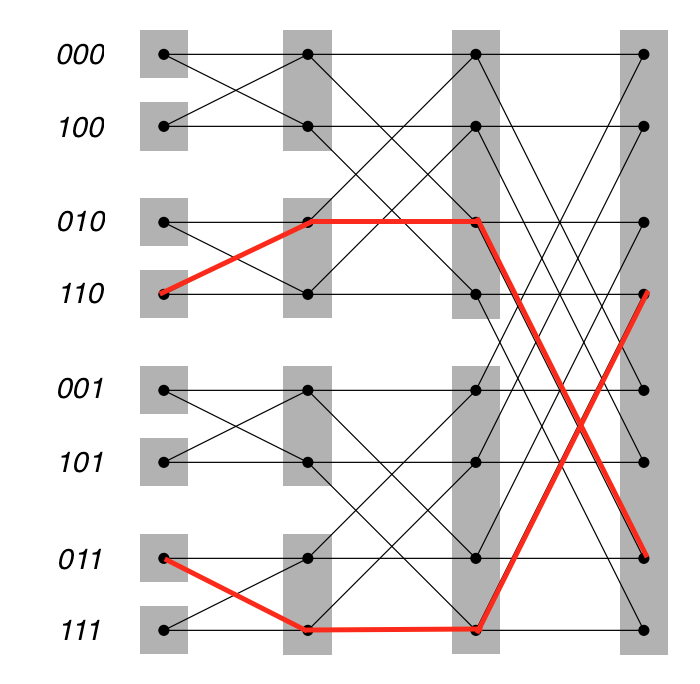
\includegraphics{butterfly-answer}
 \end{center}
 \end{Answer}

\end{Parts}

%%%%%%%%%%%%%%%%%%%% QUESTIONS END HERE

\end{document}